\documentclass[../../../main.tex]{subfiles}
\begin{document}

%%%%%%%%%%%%%%%%%%%%%%%%%%%%%%%%%%%%%%%%%
%%%%%%%%%%%%%%%%%%%%%%%%%%%%%%%%%%%%%%%%%
%%%%%%%%%%%%%%%%%%%%%%%%%%%%%%%%%%%%%%%%%
\chapter{The binomial distribution}

Consider the following set up:

\begin{itemize}
  \item Suppose we have an experiment, each repetition of which is independent. For example, flipping a coin. 
  \item Now suppose we consider one particular outcome a \vocab{success}, and we consider any other outcome a \vocab{failure}. (Don't think of success or failure as good or bad. ``Success'' is just the outcome we want to focus on.) So, the idea is that we can run the experiment (we can flip a coin), and we either succeed or we don't. For instance, we could say that in our coin flip, getting heads is ``success,'' and so each time we flip the coin, we either succeed (we get heads), or we don't. 
  \item Now suppose we want to run this experiment a certain number of times. Each run of the experiment is called a \vocab{trial}. So, for instance, say we want 3 trials, i.e., we want to flip the coin three times.
  \item Finally, the random variable $\RandVar/$ we want to know is: ``how many successes did we get in $\numTrials/$ trials?''
\end{itemize}

\noindent
What are all the results that we could get? That is, what is each possible value $\RandVarVal/$ that $\RandVarVal/$ could take on? Here are the possible values:

\begin{itemize}
  \item We could have 0 successes out of the three trials (we could get all tails). So $x$ could be 0.
  \item We could have 1 success out of the three trials (we could get heads once). So $x$ could be 1.
  \item We could have 2 successes (we could get heads twice). So $x$ could also be 2.
  \item We could have 3 successes (we could get heads all three times). So $x$ could even be 3.
\end{itemize}

What are the probabilities of all these outcomes? If we calculate these probabilities and make a \PDFtext/ for them, we will have constructed a binomial probability distribution. A binomial distribution is just a \PDFtext/ that handles exactly this sort of scenario.


%%%%%%%%%%%%%%%%%%%%%%%%%%%%%%%%%%%%%%%%%
%%%%%%%%%%%%%%%%%%%%%%%%%%%%%%%%%%%%%%%%%
\section{Definition}

A \vocab{binomial probability distribution} (or a ``binomial distribution'' for short) is a \PDFtext/ for an experiment such that:

\begin{itemize}
  \item There are $\numTrials/$ trials of the experiment.
  \item Each run of the experiment is independent (so sampling must be done with replacement).
  \item There are only two possible outcomes for each trial: either ``success'' or ``failure'' (no outcome is neutral). So, the probability of success (call it $\success/$) for a trial and the probability of failure (call it $\failure/$) for a trial should add up to 1 (100\%). Whatever the probability of success is (namely, $\success/$), the probability of failure ($\failure/$) is $1 - p$.
  \item The values that $\RandVarVal/$ can take on (namely, the number of successful trials) is distrete.
\end{itemize}


%%%%%%%%%%%%%%%%%%%%%%%%%%%%%%%%%%%%%%%%%
%%%%%%%%%%%%%%%%%%%%%%%%%%%%%%%%%%%%%%%%%
\section{Example 1}

Let the experiment be flipping a coin, and let getting heads count as success. Let there be 3 trials. What is the binomial distribution for this?

Let's calculate all the outcomes by hand. 


%%%%%%%%%%%%%%%%%%%%%%%%%%%%%%%%%%%%%%%%%
\subsection{Zero successes}

First, let's consider the case where we have 0 successes. How many ways are there to get zero successes in 3 trials? There is only 1 way: namely, if we flip tails every time. Here it is as a (one-rowed) table:

\begin{center}
  \begin{tabular}{| c | c | c | c |}
    \hline
    \textbf{Trial} & \textbf{1} & \textbf{2} & \textbf{3} \\ \hline
    Outcome & F & F & F \\ \hline
  \end{tabular}
\end{center}

\noindent
So, the number of ways to get 0 out of 3 is 1. 

Notice that this is just $\combs{0}{3}$. That is to say, we are saying: how many ways can we get 0 of 3? Well, there's only one way, namely by getting none of them.

Let's rewrite the above table, and put probabilities into it instead of success or failure. What is the probability of success $\success/$? Well, the probability of getting heads on a coin flip is .5, so:

\begin{equation*}
    p = 0.5
\end{equation*}

\noindent
The probability of failure $\failure/$ is thus $1 - p$, so:

\begin{equation*}
    q = 1 - p = 1 - 0.5 = 0.5
\end{equation*}

\noindent
And of course, that makes sense, because the probability of flipping a tails is also .5. That's why we say it's 50/50. We divide 100 up into two equal parts: half of the probability is for getting heads, and the other half of the probability is for getting tails.

Now, let's write the table again, but replace every ``S'' with the value of $\success/$, and every ``F'' with the value of $\failure/$. There are no successes here, so we just replace every ``F'' with the value of $\failure/$, which is 0.5:

\begin{center}
  \begin{tabular}{| c | c | c | c |}
    \hline
    \textbf{Trial} & \textbf{1} & \textbf{2} & \textbf{3} \\ \hline
    Outcome & 0.5 & 0.5 & 0.5 \\ \hline
  \end{tabular}
\end{center}

\noindent
Now, what is the total probability of getting this particular outcome (i.e., of getting all failures)? We just multiply the probabilities together: $0.5 * 0.5 * 0.5$, which is $0.125$:

\begin{center}
  \begin{tabular}{| c | c | c | c | c |}
    \hline
    \textbf{Trial} & \textbf{1} & \textbf{2} & \textbf{3} & \textbf{Probability} \\ \hline
    Outcome & 0.5 & 0.5 & 0.5 & 0.125 \\ \hline
  \end{tabular}
\end{center}

\noindent
So, the probability of getting 0 successes out of 3 trials is 0.125.


%%%%%%%%%%%%%%%%%%%%%%%%%%%%%%%%%%%%%%%%%
\subsubsection{Start building a formula}

Before we move on, let us start to build a formula that lets us calculate that probability. What did we do here? Well, we have $\numTrials/$ trials. In each column, we have a probability. The probability is either $\success/$ or $\failure/$. And then we multiply those together. In this case, we have 3 failures, so we multiply $\failure/$ three times:

\begin{equation*}
  q * q * q
\end{equation*}

But that's the same as:

\begin{equation*}
  q^{3}
\end{equation*}

In other words, this is $\failure/$ raised to the power of however many failures there are (in this case 3).

So, we could say that we calculate the probability like this:

\begin{equation*}
  \Pdf{x = 0} = q^{text{num failures}}
\end{equation*}


%%%%%%%%%%%%%%%%%%%%%%%%%%%%%%%%%%%%%%%%%
\subsection{One success}

Now, let's consider the case where we have 1 success. There are three different ways we can get one success: either we get heads on the first trial, or in the second trial, or in the third trial. Here they are:

\begin{center}
  \begin{tabular}{| c | c | c | c |}
    \hline
      \textbf{Trial} & \textbf{1} & \textbf{2} & \textbf{3} \\ \hline
      Outcome & S & F & F \\ \hline
      Outcome & F & S & F \\ \hline
      Outcome & F & F & S \\ \hline
  \end{tabular}
\end{center}

\noindent
So, there are 3 ways to get 1 success in three trials.

Again, notice that this is just $\combs{1}{3}$. That is to say, we are saying: how many ways can we get 1 out of 3? Well, there are 3: either we get the first, or the second, or the third.

Let's write that table again, but replace every ``S'' with the value of $\success/$, and every ``F'' with the value of $\failure/$. To help us remember where the successes are, we'll put those in bold:

\begin{center}
  \begin{tabular}{| c | c | c | c |}
    \hline
      \textbf{Trial} & \textbf{1} & \textbf{2} & \textbf{3} \\ \hline
  Outcome & \textbf{0.5} & 0.5 & 0.5 \\ \hline
  Outcome & 0.5 & \textbf{0.5} & 0.5 \\ \hline
  Outcome & 0.5 & 0.5 & \textbf{0.5} \\ \hline
  \end{tabular}
\end{center}

\noindent
What is the total probability for each row? We just multiply the probabilities together: $0.5 * 0.5 * 0.5$, which again is $0.125$:

\begin{center}
  \begin{tabular}{| c | c | c | c | c |}
    \hline
    \textbf{Trial} & \textbf{1} & \textbf{2} & \textbf{3} & \textbf{Probability} \\ \hline
  Outcome & \textbf{0.5} & 0.5 & 0.5 & 0.125 \\ \hline
  Outcome & 0.5 & \textbf{0.5} & 0.5 & 0.125 \\ \hline
  Outcome & 0.5 & 0.5 & \textbf{0.5} & 0.125 \\ \hline
  \end{tabular}
\end{center}

\noindent
But there's something new here that wasn't present in the last case, when we were calculating the probability of getting 0 successes in 3 trials. In this case, there's not just one row here. There are three rows. In other words, there is not just one way to get a single success. There are actually 3 ways. 

In the last case, when we calculated the probability of getting 0 successes out of 3 trials, we saw that there was only one way to get that result. But here there are 3 ways. So the total probability of getting one success out of 3 trials is 3 times greater. In other words, we need to multiply the probability of one row by the number of rows.

So, the total probability of getting 1 success out of 3 trials is this:

\begin{equation*}
    3 * 0.125 = 0.375
\end{equation*}


%%%%%%%%%%%%%%%%%%%%%%%%%%%%%%%%%%%%%%%%%
\subsubsection{Improve the formula}

Let's try and improve our formula to calculate the probability. Let's look at the first row of this column. We calculated the probability by multiplying the probabilities of each column. What is in the first column? Well, we have one $\success/$ (one success), and 2 $\failure/$s (two failures):

\begin{equation*}
    p * q * q
\end{equation*}

That's the same as this:

\begin{equation*}
   p^{1} * q^{2}
\end{equation*}

And that's the same as this:

\begin{equation*}
   p^{\text{num success}} * q^{\text{num failures}}
\end{equation*}

Does this work for each row? Look at the second row. We have failure, success, then failure:

\begin{equation*}
   q * p * q
\end{equation*}

But if we reorder these, that's the same as:

\begin{equation*}
   p * q * q
\end{equation*}

And that's the same as:

\begin{equation*}
   p^{1} * q^{2}
\end{equation*}

Which again is the same as this:

\begin{equation*}
   p^{\text{num success}} * q^{\text{num failures}}
\end{equation*}

So the same formula works for the second row.

What about the third row? We have two failures and one success:

\begin{equation*}
    q * q * p
\end{equation*}

Rearranged, we get:

\begin{equation*}
    p * q * q
\end{equation*}

Which is:

\begin{equation*}
   p^{1} * q^{2}
\end{equation*}

And that is again the same as:

\begin{equation*}
   p^{\text{num success}} * q^{\text{num failures}}
\end{equation*}

So the same formula works for the third row too. We can thus use this formula to calculate the probability of each row. 

But then we have 3 rows. So we have to multiply that by 3:

\begin{equation*}
    3 * p^{\text{num success}} * q^{\text{num failures}}
\end{equation*}

What's 3? It's the number of combinations. So, we can rewrite the formula like this:

\begin{equation*}
    \text{num combinations } * p^{\text{num success}} * q^{\text{num failures}}
\end{equation*}


%%%%%%%%%%%%%%%%%%%%%%%%%%%%%%%%%%%%%%%%%
\subsection{Two successes}

Now, let's consider the case where we have 2 success. There are three different ways we can get two successes: either we get heads in the first two trials, or in the last two trials, or in the first and third trial. Here they are:

\begin{center}
  \begin{tabular}{| c | c | c | c |}
    \hline
      \textbf{Trial} & \textbf{1} & \textbf{2} & \textbf{3} \\ \hline
    Trial & 1 & 2 & 3 \\ \hline
  Outcome & S & S & F \\ \hline
  Outcome & F & S & S \\ \hline
  Outcome & S & F & S \\ \hline
  \end{tabular}
\end{center}

\noindent
So, there are 3 ways to get 2 successes in three trials.

Again, notice that this is just $\combs{2}{3}$. That is to say, we are saying: how many ways can we get 2 out of 3? Well, there are 3: either we get the first two, or the last two, or the first and the third.

Let's rewrite the table again, but with the probabilities instead of ``S'' and ``F'':

\begin{center}
  \begin{tabular}{| c | c | c | c |}
    \hline
      \textbf{Trial} & \textbf{1} & \textbf{2} & \textbf{3} \\ \hline
  Outcome & \textbf{0.5} & \textbf{0.5} & 0.5 \\ \hline
  Outcome & 0.5 & \textbf{0.5} & \textbf{0.5} \\ \hline
  Outcome & \textbf{0.5} & 0.5 & \textbf{0.5} \\ \hline
  \end{tabular}
\end{center}

\noindent
What is the total probability for each row? We just multiply the probabilities together: $0.5 * 0.5 * 0.5$, which again is $0.125$:

\begin{center}
  \begin{tabular}{| c | c | c | c | c |}
    \hline
      \textbf{Trial} & \textbf{1} & \textbf{2} & \textbf{3} & \textbf{Probability} \\ \hline
  Outcome & \textbf{0.5} & \textbf{0.5} & 0.5 & 0.125  \\ \hline
  Outcome & 0.5 & \textbf{0.5} & \textbf{0.5} & 0.125 \\ \hline
  Outcome & \textbf{0.5} & 0.5 & \textbf{0.5} & 0.125 \\ \hline
  \end{tabular}
\end{center}

\noindent
So the probability of the trials turning out as they do in each row is 0.125. But there are 3 rows, so we need to multiply 0.125 by 3:

\begin{equation*}
    3 * 0.125 = 0.375
\end{equation*}


%%%%%%%%%%%%%%%%%%%%%%%%%%%%%%%%%%%%%%%%%
\subsubsection{Improving the formula}

Let's check that our formula works for this case. We said before that we can calculate the probability of each row like this:

\begin{equation*}
    p^{\text{num success}} * q^{\text{num failures}}
\end{equation*}

Look at the first row. Does this work? In the first row, we have two successes and one failure:

\begin{equation*}
    p * p * q
\end{equation*}

That's the same as this:

\begin{equation*}
    p^{2} * q^{1}
\end{equation*}

And since 2 is the number of successes while 1 is the number of failures, that's the same as this:

\begin{equation*}
    p^{\text{num success}} * q^{\text{num failures}}
\end{equation*}

Hence, the formula works for the first row. What about the second row? There is one failure and two successes:

\begin{equation*}
    q * p * p
\end{equation*}

Rerranged:

\begin{equation*}
    p * p * q
\end{equation*}

Which again is:

\begin{equation*}
    p^{2} * q^{1}
\end{equation*}

So the formula works for the second row too. What about the third row? We have a success, a failure, and a success:

\begin{equation*}
    p * q * p
\end{equation*}

Rerranged:

\begin{equation*}
    p * p * q
\end{equation*}

Which again is:

\begin{equation*}
    p^{2} * q^{1}
\end{equation*}

So the formula works for the third row too.

And of course, there are three rows here, so if we multiply it by the number of rows/combinations, we get:

\begin{equation*}
    \text{num combinations } * p^{\text{num success}} * q^{\text{num failures}}
\end{equation*}

So the formula works here too.


%%%%%%%%%%%%%%%%%%%%%%%%%%%%%%%%%%%%%%%%%
\subsection{Three successes}

Finally, et's consider the case where we get 3 successes. How many ways are there to get 3 successes in 3 trials? There is only 1 way: namely, if we flip heads every time. Here it is as a table:

\begin{center}
  \begin{tabular}{| c | c | c | c |}
    \hline
      \textbf{Trial} & \textbf{1} & \textbf{2} & \textbf{3} \\ \hline
    Trial & 1 & 2 & 3 \\ \hline
  Outcome & S & S & S \\ \hline
  \end{tabular}
\end{center}

\noindent
So, the number of ways to get 3 out of 3 is 1.

Again, this is just $\combs{3}{3}$. That is to say, we are saying: how many ways can we get 3 of 3? Well, there's only one way, namely by getting all of them.

Let's rewrite the table again, but with the probabilities instead of ``S'' and ``F'':

\begin{center}
  \begin{tabular}{| c | c | c | c |}
    \hline
      \textbf{Trial} & \textbf{1} & \textbf{2} & \textbf{3} \\ \hline
  Outcome & \textbf{0.5} & \textbf{0.5} & \textbf{0.5} \\ \hline
  \end{tabular}
\end{center}

\noindent
What is the total probability for this row? Again, we multiply the probabilities together: $0.5 * 0.5 * 0.5$, which again is $0.125$:

\begin{center}
  \begin{tabular}{| c | c | c | c | c |}
    \hline
      \textbf{Trial} & \textbf{1} & \textbf{2} & \textbf{3} & \textbf{Probability} \\ \hline
  Outcome & \textbf{0.5} & \textbf{0.5} & \textbf{0.5} & 0.125 \\ \hline
  \end{tabular}
\end{center}

%%%%%%%%%%%%%%%%%%%%%%%%%%%%%%%%%%%%%%%%%
\subsubsection{Improving the formula}

The formula we've got is this:

\begin{equation*}
    \text{num combinations } * p^{\text{num success}} * q^{\text{num failures}}
\end{equation*}

Does this work here too? Yes it does. We have three successes:

\begin{equation*}
    p * p * p
\end{equation*}

Which is the same as:

\begin{equation*}
    p^{3}
\end{equation*}

We have no failures, so we could say:

\begin{equation*}
    p^{3} * q^{0}
\end{equation*}

Which is the same as:

\begin{equation*}
    p^{\text{num success}} * q^{\text{num failures}}
\end{equation*}

Finally, we have one row, so we could say:

\begin{equation*}
    1 * p^{\text{num success}} * q^{\text{num failures}}
\end{equation*}

And that's the same as:

\begin{equation*}
    \text{num combinations } * p^{\text{num success}} * q^{\text{num failures}}
\end{equation*}

So the formula works here too.


%%%%%%%%%%%%%%%%%%%%%%%%%%%%%%%%%%%%%%%%%
\subsection{A table}

Let's put all these results together in a table. We put the number of the trial in the first column, the number of successes and failures in the next two columns, then we put the combination formula in the next column, and we put the computed total number of combinations for that row in the last column.

\begin{center}
  \begin{tabular}{| c | c | c | c | c |}
    \hline
  \textbf{n} & \textbf{Succ} & \textbf{Fail} & \textbf{Comb} & \textbf{Total} \\ \hline
  0 & 0    & 3    & $\combs{0}{3}$ & 1 \\ \hline
  1 & 1    & 2    & $\combs{1}{3}$ & 2 \\ \hline
  2 & 2    & 1    & $\combs{2}{3}$ & 2 \\ \hline
  3 & 3    & 0    & $\combs{3}{3}$ & 1 \\ \hline
  \end{tabular}
\end{center}

\noindent
Let's rewrite this with the probabilities:

\begin{center}
  \begin{tabular}{| c | c | c | c | c |}
    \hline
  \textbf{n} & \textbf{Succ} & \textbf{Fail} & \textbf{Comb} & \textbf{Total} \\ \hline
  0 & 0    & 3    & $\combs{0}{3}$ & 0.125 \\ \hline
  1 & 1    & 2    & $\combs{1}{3}$ & 0.375 \\ \hline
  2 & 2    & 1    & $\combs{2}{3}$ & 0.375 \\ \hline
  3 & 3    & 0    & $\combs{3}{3}$ & 0.125 \\ \hline
  \end{tabular}
\end{center}

\noindent
Notice that the probabilities all add up to 1:

\begin{equation*}
    0.125 + 0.375 + 0.375 + 0.125 = 1
\end{equation*}

\noindent
Let's plot it. See Figure \ref{plot:example-1}.

\begin{figure}[ht]
  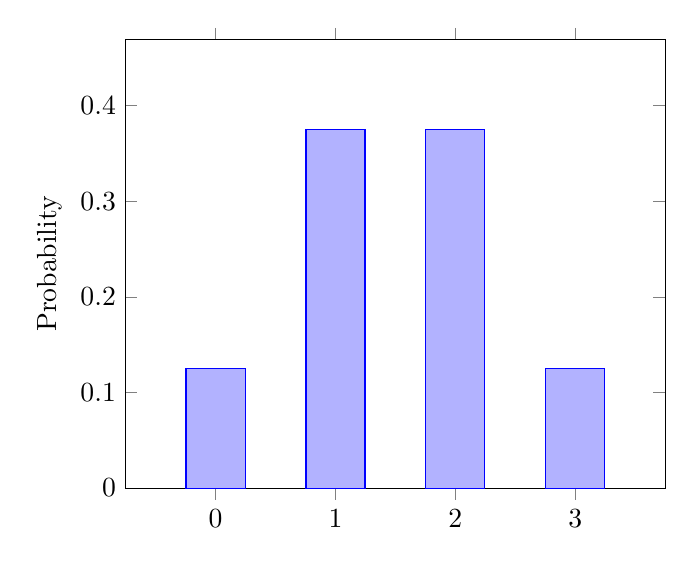
\begin{tikzpicture}
    \centering
    \begin{axis} [
      ylabel=Probability,
      symbolic x coords={0, 1, 2, 3},
      ybar,
      xtick=data,
      ymin=0,
      enlarge y limits={value=0.25,upper},
      enlarge x limits=0.25,
      % nodes near coords,
      bar width=0.75cm,
      ]
      \addplot coordinates {(0, 0.125) (1, 0.375) (2, 0.375) (3, 0.125)};
    \end{axis}
  \end{tikzpicture}
  \caption{\label{plot:example-1} $\Probability{\RandVarVal/}$}
\end{figure}

Where are the probabilities distributed? We can see that most of the probability is chunked in the middle, around getting 1 or 2 successes. 

If you think about it, this makes sense. The probability of getting 1 or 2 successes should be greater than getting either no successes at all or getting all successes. It should be much rarer that you get no successes or all successes.


%%%%%%%%%%%%%%%%%%%%%%%%%%%%%%%%%%%%%%%%%
\subsection{The formula}

Earlier, we figured out that the formula is this:

\begin{equation*}
    \text{num combinations } * p^{\text{num success}} * q^{\text{num failures}}
\end{equation*}

Let's replace the English words ``num combinations,'' ``num success,'' and ``num failures'' with something more exact.

\begin{itemize}
  \item What's the ``num success''? Well, it's $\RandVarVal/$. So the equation is: $\text{num combinations } * p^{\RandVarVal/} * q^{\text{num failures}}$
  \item What's the ``num failures''? It's however many of $\numTrials/$ are left after we get the successes $\RandVarVal/$. So it's $n - \RandVarVal/$. Hence, the equation is: $\text{num combinations } * p^{\RandVarVal/} * q^{n - \RandVarVal/}$.
  \item What's the ``num combinations''? Well, it's the number of successes $\RandVarVal/$ out of the number of trials $\numTrials/$. So it's $\combs{\RandVarVal/}{n}$. Hence, the equation is: $\combs{\RandVarVal/}{n} * p^{\RandVarVal/} * q^{n - \RandVarVal/}$.
\end{itemize}

\noindent
And with that, we have the fully general formula to calculate the probability for any given number of successes $\RandVarVal/$ out of $\numTrials/$ trials. Let's call the binomial \PDFtext/ this: 

\begin{equation*}
    \Binom{\RandVarVal/}
\end{equation*}

Hence, we can write the full formula like this:

\begin{equation*}
    \Binom{\RandVarVal/} = \combs{\RandVarVal/}{n} * p^{\RandVarVal/} * q^{n - \RandVarVal/}
\end{equation*}

Notice that you need to know $\success/$, $\failure/$, $\numTrials/$, and $x$. If you know those values, you can plug them in to this formula, and you'll get the probability you want. 

Of course, you \emph{could} construct the tables yourself as we did here, but this formula is often much quicker. Building the table is useful if you want to check your work, and it's especially useful when you want to make sure you understand the experiment.


%%%%%%%%%%%%%%%%%%%%%%%%%%%%%%%%%%%%%%%%%
%%%%%%%%%%%%%%%%%%%%%%%%%%%%%%%%%%%%%%%%%
\section{Example 2}

Suppose we have a bag of 5 marbles. 3 are red, 1 is blue, and 1 is green. Let the experiment be pulling a marble out of the bag (and then replacing it). Let ``success'' be pulling out a red marble. 

Now, let there be 4 trials. What is the binomial distribution this?

Here is what we know:

\begin{itemize}
  \item $\RandVarVal/$ is 0, 1, 2, 3, and 4. That is, there is the case where we get 0 successes, 1 success, 2 successes, 3 successes, and 4 successes.
  \item $\numTrials/$ is 4. We want to run 4 trials (we want to draw 4 marbles, with replacement).
\end{itemize}

We need to know $\success/$ and $\failure/$, so we need to calculate them.

\begin{itemize}
  \item $\success/$ is drawing a red marble, and 3 of the 5 marbles are red. So $\success/ = \frac{3}{5} = 0.6$.
  \item $\failure/$ is not drawing a red marble. It's got to be $1 - p$, which is $0.4$. This makes sense, because there are only 2 marbles that aren't red, and 2 of 5 is $\frac{2}{5} = 0.4$.
\end{itemize}

Let's calculate all the outcomes by hand, and then we'll use the formula to confirm.


%%%%%%%%%%%%%%%%%%%%%%%%%%%%%%%%%%%%%%%%%
\subsection{Zero successes}

First, let's consider the case where we have 0 successes. How many ways are there to get zero successes in 4 trials? There is one way: if on each trial, we pull out a blue or green (i.e., a marble that is not red). Here it is:

\begin{center}
  \begin{tabular}{| c | c | c | c | c |}
    \hline
    \textbf{Trial} & \textbf{1} & \textbf{2} & \textbf{3} & \textbf{4} \\ \hline
  Outcome & F & F & F & F \\ \hline
  \end{tabular}
\end{center}

\noindent
So, the number of ways to get 0 out of 4 is 1. That's the same as $\combs{0}{4}$. 

Let's rewrite the table, with $\success/$ and $\failure/$ values instead of ``S'' and ``F'':

\begin{center}
  \begin{tabular}{| c | c | c | c | c | c |}
    \hline
    \textbf{Trial} & \textbf{1} & \textbf{2} & \textbf{3} & \textbf{4} & \textbf{Probability} \\ \hline
  Outcome & 0.4 & 0.4 & 0.4 & 0.4 & 0.0256 \\ \hline
  \end{tabular}
\end{center}

\noindent
The formula gives us the same result:

\begin{equation*}
  \Binom{\RandVarVal/} = \combs{\RandVarVal/}{n} * p^{\RandVarVal/} * q^{n - \RandVarVal/} = 1 * 0.6^{0} * 0.4^{4} = 0.0256
\end{equation*}


%%%%%%%%%%%%%%%%%%%%%%%%%%%%%%%%%%%%%%%%%
\subsection{One success}

How many ways are there to get one success in 4 trials? There are four ways: we get a success on the first trial, the second trial, the third trial, or the fourth trial:

\begin{center}
  \begin{tabular}{| c | c | c | c | c |}
    \hline
    \textbf{Trial} & \textbf{1} & \textbf{2} & \textbf{3} & \textbf{4} \\ \hline
    Trial & 1 & 2 & 3 & 4 \\ \hline
  Outcome & S & F & F & F \\ \hline
  Outcome & F & S & F & F \\ \hline
  Outcome & F & F & S & F \\ \hline
  Outcome & F & F & F & S \\ \hline
  \end{tabular}
\end{center}

\noindent
So, the number of ways to get 1 out of 4 is 4. That's the same as $\combs{1}{4}$. 

Let's rewrite the table, with $\success/$ and $\failure/$ values instead of ``S'' and ``F'':

\begin{center}
  \begin{tabular}{| c | c | c | c | c | c |}
    \hline
    \textbf{Trial} & \textbf{1} & \textbf{2} & \textbf{3} & \textbf{4} & \textbf{Probability} \\ \hline
  Outcome & 0.6 & 0.4 & 0.4 & 0.4 & 0.0384 \\ \hline
  Outcome & 0.4 & 0.6 & 0.4 & 0.4 & 0.0384 \\ \hline
  Outcome & 0.4 & 0.4 & 0.6 & 0.4 & 0.0384 \\ \hline
  Outcome & 0.4 & 0.4 & 0.4 & 0.6 & 0.0384 \\ \hline
  \end{tabular}
\end{center}

\noindent
And if we multiply 0.0384 by the number of rows/combinations (which is 4), we get:

\begin{equation*}
    4 * 0.0384 = 0.1536
\end{equation*}

The formula gives us the same result:

\begin{equation*}
  \Binom{\RandVarVal/} = \combs{\RandVarVal/}{n} * p^{\RandVarVal/} * q^{n - \RandVarVal/} = 1 * 0.6^{0} * 0.4^{4} = 0.1536
\end{equation*}


%%%%%%%%%%%%%%%%%%%%%%%%%%%%%%%%%%%%%%%%%
\subsection{Two successes}

How many ways are there to get two successes in 4 trials? There are six ways:

\begin{center}
  \begin{tabular}{| c | c | c | c | c |}
    \hline
    \textbf{Trial} & \textbf{1} & \textbf{2} & \textbf{3} & \textbf{4} \\ \hline
  Outcome & S & S & F & F \\ \hline
  Outcome & S & F & S & F \\ \hline
  Outcome & S & F & F & S \\ \hline
  Outcome & F & S & S & F \\ \hline
  Outcome & F & S & F & S \\ \hline
  Outcome & F & F & S & S \\ \hline
  \end{tabular}
\end{center}

\noindent
So, the number of ways to get 2 out of 4 is 6. That's the same as $\combs{2}{4}$. 

Let's rewrite the table, with $\success/$ and $\failure/$ values instead of ``S'' and ``F'':

\begin{center}
  \begin{tabular}{| c | c | c | c | c | c |}
    \hline
    \textbf{Trial} & \textbf{1} & \textbf{2} & \textbf{3} & \textbf{4} & \textbf{Probability} \\ \hline
  Outcome & 0.6 & 0.6 & 0.4 & 0.4 & 0.0576 \\ \hline
  Outcome & 0.6 & 0.4 & 0.6 & 0.4 & 0.0576 \\ \hline
  Outcome & 0.6 & 0.4 & 0.4 & 0.6 & 0.0576 \\ \hline
  Outcome & 0.4 & 0.6 & 0.6 & 0.4 & 0.0576 \\ \hline
  Outcome & 0.4 & 0.6 & 0.4 & 0.6 & 0.0576 \\ \hline
  Outcome & 0.4 & 0.4 & 0.6 & 0.6 & 0.0576 \\ \hline
  \end{tabular}
\end{center}

\noindent
And if we multiply 0.0576 by the number of rows/combinations (which is 6), we get:

\begin{equation*}
    6 * 0.0576 = 0.3456
\end{equation*}

\noindent
The formula gives us the same result:

\begin{equation*}
  \Binom{\RandVarVal/} = \combs{\RandVarVal/}{n} * p^{\RandVarVal/} * q^{n - \RandVarVal/} = 1 * 0.6^{0} * 0.4^{4} = 0.3456
\end{equation*}


%%%%%%%%%%%%%%%%%%%%%%%%%%%%%%%%%%%%%%%%%
\subsection{Three successes}

How many ways are there to get three successes in 4 trials? There are 4 ways:

\begin{center}
  \begin{tabular}{| c | c | c | c | c |}
    \hline
    \textbf{Trial} & \textbf{1} & \textbf{2} & \textbf{3} & \textbf{4} \\ \hline
  Outcome & S & S & S & F \\ \hline
  Outcome & S & S & F & S \\ \hline
  Outcome & S & F & S & S \\ \hline
  Outcome & F & S & S & S \\ \hline
  \end{tabular}
\end{center}

\noindent
And here are those two rows with the probabilities filled in:

\begin{center}
  \begin{tabular}{| c | c | c | c | c | c |}
    \hline
    \textbf{Trial} & \textbf{1} & \textbf{2} & \textbf{3} & \textbf{4} & \textbf{Probability} \\ \hline
  Outcome & 0.6 & 0.6 & 0.6 & 0.4 & 0.0864 \\ \hline
  Outcome & 0.6 & 0.6 & 0.4 & 0.6 & 0.0864 \\ \hline
  Outcome & 0.6 & 0.4 & 0.6 & 0.6 & 0.0864 \\ \hline
  Outcome & 0.4 & 0.6 & 0.6 & 0.6 & 0.0864 \\ \hline
  \end{tabular}
\end{center}

\noindent
And if we multiply that by the number of rows/combinations (which is 4), we get:

\begin{equation*}
    4 * 0.0864 = 0.3456
\end{equation*}

\noindent
The formula gives us the same result:

\begin{equation*}
  \Binom{\RandVarVal/} = \combs{\RandVarVal/}{n} * p^{\RandVarVal/} * q^{n - \RandVarVal/} = 1 * 0.6^{0} * 0.4^{4} = 0.3456
\end{equation*}


%%%%%%%%%%%%%%%%%%%%%%%%%%%%%%%%%%%%%%%%%
\subsection{Four successes}

How many ways are there to get 4 successes in 4 trials? There is one way: you get a success every time.

\begin{center}
  \begin{tabular}{| c | c | c | c | c |}
    \hline
    \textbf{Trial} & \textbf{1} & \textbf{2} & \textbf{3} & \textbf{4} \\ \hline
  Outcome & S & S & S & S \\ \hline
  \end{tabular}
\end{center}

\noindent
So, the number of ways to get 4 out of 4 is 1. That's the same as $\combs{4}{4}$. 

Let's rewrite the table, with $\success/$ and $\failure/$ values instead of ``S'' and ``F'':

\begin{center}
  \begin{tabular}{| c | c | c | c | c | c |}
    \hline
    \textbf{Trial} & \textbf{1} & \textbf{2} & \textbf{3} & \textbf{4} & \textbf{Probability} \\ \hline
  Outcome & 0.6 & 0.6 & 0.6 & 0.6 & 0.1296 \\ \hline
  \end{tabular}
\end{center}

\noindent
And if we multiply 0.1296 by the number of rows/combinations (which is 1), we get:

\begin{equation*}
    1 * 0.1296 = 0.1296
\end{equation*}

The formula gives us the same result:

\begin{equation*}
  \Binom{\RandVarVal/} = \combs{\RandVarVal/}{n} * p^{\RandVarVal/} * q^{n - \RandVarVal/} = 1 * 0.6^{0} * 0.4^{4} = 0.1296
\end{equation*}


%%%%%%%%%%%%%%%%%%%%%%%%%%%%%%%%%%%%%%%%%
\subsection{One big table}

Let's take these results and put them together to build our binomial \PDFtext/ function/table:

\begin{center}
  \begin{tabular}{| c | c | c | c | c |}
    \hline
  \textbf{n} & \textbf{Succ} & \textbf{Fail} & \textbf{Comb} & \textbf{Total} \\ \hline
  0 & 0    & 4    & $\combs{0}{4}$ & 1 \\ \hline
  1 & 1    & 3    & $\combs{1}{4}$ & 4 \\ \hline
  2 & 2    & 2    & $\combs{2}{4}$ & 6 \\ \hline
  3 & 3    & 1    & $\combs{3}{4}$ & 4 \\ \hline
  4 & 4    & 0    & $\combs{4}{4}$ & 1 \\ \hline
  \end{tabular}
\end{center}

\noindent
Let's rewrite this with the probabilities:

\begin{center}
  \begin{tabular}{| c | c | c | c | c |}
    \hline
  \textbf{n} & \textbf{Succ} & \textbf{Fail} & \textbf{Comb} & \textbf{Total} \\ \hline
  0 & 0    & 4    & $\combs{0}{4}$ & 0.0256 \\ \hline
  1 & 1    & 3    & $\combs{1}{4}$ & 0.1536 \\ \hline
  2 & 2    & 2    & $\combs{2}{4}$ & 0.3456 \\ \hline
  3 & 3    & 1    & $\combs{3}{4}$ & 0.3456 \\ \hline
  4 & 4    & 0    & $\combs{4}{4}$ & 0.1296 \\ \hline
  \end{tabular}
\end{center}

\noindent
Notice that the probabilities all add up to 1:

\begin{equation*}
    0.0256 + 0.1536 + 0.3456 + 0.3456 + 0.1296 = 1
\end{equation*}

\noindent
Let's plot it. See Figure \ref{plot:example-2}.

\begin{figure}[ht]
  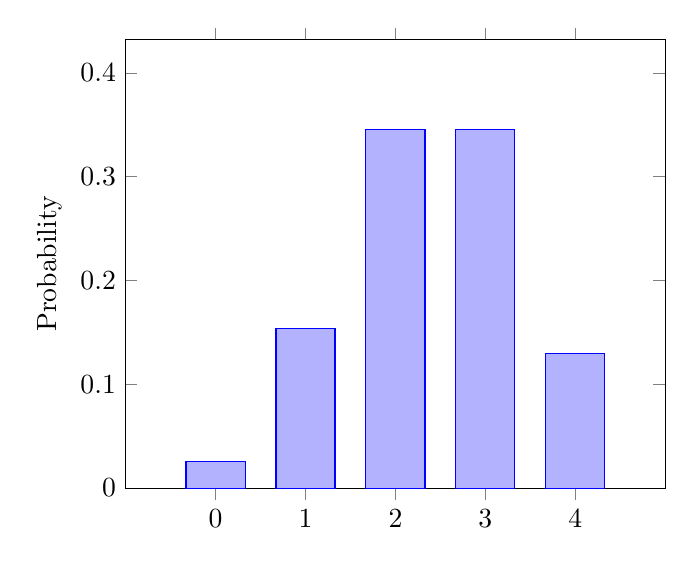
\begin{tikzpicture}
    \centering
    \begin{axis} [
      ylabel=Probability,
      symbolic x coords={0, 1, 2, 3, 4},
      ybar,
      xtick=data,
      ymin=0,
      enlarge y limits={value=0.25,upper},
      enlarge x limits=0.25,
      % nodes near coords,
      bar width=0.75cm,
      ]
      \addplot coordinates {(0, 0.0256) (1, 0.1536) (2, 0.3456) (3, 0.3456) (4, 0.1296)};
    \end{axis}
  \end{tikzpicture}
  \caption{\label{plot:example-2} $\Probability{\RandVarVal/}$}
\end{figure}

Where are the probabilities distributed? We can see that most of the probability is chunked in the middle, and it tapers off at the edges. 

Again, this makes sense. The probability of getting a mixture of successes is greater than getting either no successes at all or getting all successes.

Notice also that the probabilities are skewed a little to the right. If you think about it, this makes sense too. The reason is that there are more red marbles in the bag than non-red marbles. So the chances of getting more successes is higher than getting fewer successes.

Look also at the two end cases: the case where you get 0 successes, and the case where you get 4 successes. The probability of getting 0 successes is lower than the probability of getting all successes. This is right, because there are more red marbles in the bag, so of these two possibilities, the chance of getting all successes is greater than the chance of getting no successes at all.

But of course, the chances of getting 1, 2, or 3 successes is still higher than getting no successes or all successes, as is the case in any binomial experiment.


%%%%%%%%%%%%%%%%%%%%%%%%%%%%%%%%%%%%%%%%%
%%%%%%%%%%%%%%%%%%%%%%%%%%%%%%%%%%%%%%%%%
\section{Example 3}

Alice is a specialist in renegotiating contracts. Looking back over the last 10 of her clients, we see that she has succeed at renegotiating a lower cost for her clients in 7 out of those 10 cases.

Let the experiment be that Alice renegotiates a contract, let ``success'' be that she succeeds at negotiating a lower cost for he client, let there be 7 trials. What is the binomial distribution for this?

Here are the values we need:

\begin{itemize}
  \item The $\RandVar/$ is getting a lower cost for her client.
  \item The values that $\RandVarVal/$ can take on are 0 through 7 (since she can succeed 0 through 7 times in 7 trials).
  \item The probability $\success/$ that she will succeed on any one trial is 7 out of 10, or .7.
  \item The probability $\failure/$ that she will fail is $1 - \success/$, or $1 - .7 = .3$.
\end{itemize}

\noindent
Let's build the binomial \PDFtext/ function/table:

\begin{center}
  \begin{tabular}{| c | c | c | c | c |}
    \hline
  \textbf{n} & \textbf{Succ} & \textbf{Fail} & \textbf{Comb} & \textbf{Total} \\ \hline
  0 & 0    & 7    & $\combs{0}{7}$ & 1 \\ \hline
  1 & 1    & 6    & $\combs{1}{7}$ & 4 \\ \hline
  2 & 2    & 5    & $\combs{2}{7}$ & 6 \\ \hline
  3 & 3    & 4    & $\combs{3}{7}$ & 4 \\ \hline
  4 & 4    & 3    & $\combs{4}{7}$ & 1 \\ \hline
  5 & 5    & 2    & $\combs{5}{7}$ & 1 \\ \hline
  6 & 6    & 1    & $\combs{6}{7}$ & 1 \\ \hline
  7 & 7    & 0    & $\combs{7}{7}$ & 1 \\ \hline
  \end{tabular}
\end{center}

\noindent
Let's rewrite this with the probabilities:

\begin{center}
  \begin{tabular}{| c | c | c | c | c |}
    \hline
  \textbf{n} & \textbf{Succ} & \textbf{Fail} & \textbf{Comb} & \textbf{Total} \\ \hline
  0 & 0    & 7    & $\combs{0}{7}$ & 0.0002 \\ \hline
  1 & 1    & 6    & $\combs{1}{7}$ & 0.0036 \\ \hline
  2 & 2    & 5    & $\combs{2}{7}$ & 0.0250 \\ \hline
  3 & 3    & 4    & $\combs{3}{7}$ & 0.0972 \\ \hline
  4 & 4    & 3    & $\combs{4}{7}$ & 0.2269 \\ \hline
  5 & 5    & 2    & $\combs{5}{7}$ & 0.3177 \\ \hline
  6 & 6    & 1    & $\combs{6}{7}$ & 0.2471 \\ \hline
  7 & 7    & 0    & $\combs{7}{7}$ & 0.0824 \\ \hline
  \end{tabular}
\end{center}

\noindent
Notice that the probabilities all add up to 1 (modulo some rounding errors):

\begin{equation*}
    0.0002 + 0.0036 + 0.025 + 0.0972 + 0.2269 + 0.3177 + 0.2471 + 0.0824 = 1
\end{equation*}

\noindent.
Let's graph it:

\noindent
Let's plot it. See Figure \ref{plot:example-3}.

\begin{figure}[ht]
  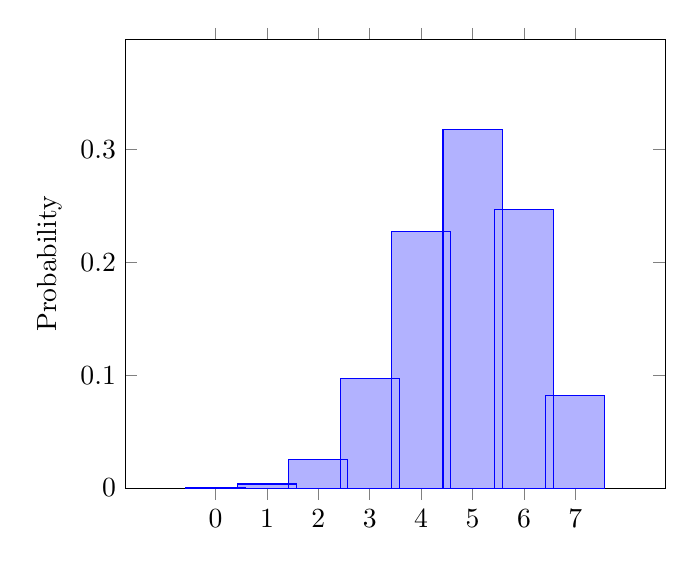
\begin{tikzpicture}
    \centering
    \begin{axis} [
      ylabel=Probability,
      symbolic x coords={0, 1, 2, 3, 4, 5, 6, 7},
      ybar,
      xtick=data,
      ymin=0,
      enlarge y limits={value=0.25,upper},
      enlarge x limits=0.25,
      % nodes near coords,
      bar width=0.75cm,
      ]
      \addplot coordinates {(0, 0.0002) (1, 0.0036) (2, 0.025) (3, 0.0972) (4, 0.2269) (5, 0.3177) (6, 0.2471) (7, 0.0824)};
    \end{axis}
  \end{tikzpicture}
  \caption{\label{plot:example-3} $\Probability{\RandVarVal/}$}
\end{figure}

Where are the probabilities distributed? We can see that most of the probability is chunked over towards the right. And this makes sense, since Alice has a pretty good success rate, so the probability of getting more successes on the trials should be higher than getting fewer successes.


\end{document}
